\emph{Author}: Joe Corneli

\href{planetmath.org}{PlanetMath} is \emph{a virtual community which aims
to help make mathematical knowledge more accessible}. This article
summarizes the main design ideas behind a complete rebuild of the
site's platform. It gets a little technical, but don't worry, there's
not too much \emph{math} here\ldots{}

In short: I lumped the different activities that people could do on
PlanetMath.org into 5 categories (see the table below). More or less
this table just means that on PlanetMath, people write articles and link
these articles to other articles, add comments, ask questions, make
corrections, and connect problems and solutions to expository material.
They also deploy
\href{http://peeragogy.org/patterns-usecases/patterns-and-heuristics/}{heuristics}
for solving problems -- and they
\href{http://peeragogy.org/convening-group/}{make and join groups}.

\begin{table}
\begin{center}
{\Tiny
\begin{tabular}{| >{\centering\arraybackslash}m{.15\textwidth} | >{\centering\arraybackslash}m{.15\textwidth} | >{\centering\arraybackslash}m{.15\textwidth} | >{\centering\arraybackslash}m{.15\textwidth} | >{\centering\arraybackslash}m{.17\textwidth}| }
\hline
Context & Feedback & Quality & Structure & Heuristic \\[.2mm]
\hline
\vspace{.2mm}
$\begin{array}{c}
A \leftarrow A \\
A \xleftarrow{\ell} A
\end{array}$
&
$\begin{array}{c}
X \leftarrow T \\
S \leftarrow R
\end{array}$  &
$\begin{array}{c}
X \leftarrow Q \\
A \leftarrow C
\end{array}$ &
$\begin{array}{c}
A \leftarrow P
\leftarrow S \\
L \leftarrow A, P \\
M \leftarrow A \\
Q \leftarrow A
\end{array}$&
$\begin{array}{c}
G \hookleftarrow U \\
S\hookleftarrow H \\
Q,T\rightharpoonup C, W, P
\end{array}$ \\
\hline
$\begin{array}{r@{\hspace{2mm}}l}
A &\mathrm{article} \\
\ell &\mathrm{link}
\end{array}$  &
$\begin{array}{r@{\hspace{2mm}}l}
X &\mathrm{object} \\
T &\mathrm{post} \\
S &\mathrm{solution} \\
R &\mathrm{review}
\end{array}$ &
$\begin{array}{r@{\hspace{2mm}}l}
Q &\mathrm{question} \\
C &\mathrm{correction}
\end{array}$
&
$\begin{array}{r@{\hspace{2mm}}l}
P &\mathrm{problem} \\
L &\mathrm{collection} \\
M &\mathrm{classific.}
\end{array}$ &
$\begin{array}{r@{\hspace{2mm}}l}
G &\mathrm{group}\\
U &\mathrm{user}\\
W &\mathrm{request} \\
H &\mathrm{heuristic}
\end{array}$
\\
\hline
\end{tabular}
}
\end{center}
\caption*{A paragogical decomposition of PlanetMath's activities: ``production rules'' in the grammar of mathematical behavior\label{activity-decomposition}}
\end{table}

The five categories (Context, Engagement, Quality, Structure, and
Heuristic) come from reflecting on the \href{http://paragogy.net}{5
paragogy principles}, and comparing them with the Martin Nowak's
\href{http://www.sciencemag.org/content/314/5805/1560.full}{5 rules for
the evolution of cooperation}, then clustering the actual activities
that people can do on PlanetMath (as well as some new planned
activities) into these categories. I also drew inspiration from the
pattern and heuristic ``language'' we developed in the peeragogy
project. I started by clustering our
\href{http://peeragogy.org/patterns-usecases/patterns-and-heuristics/}{pattern
language diagram} into 5 segments, like this:

\begin{center}
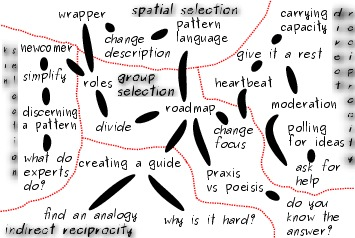
\includegraphics[width=.7\textwidth]{../pictures/subway-redline.jpg}
\end{center}
The ``key'' that shows how things fit together is as follows:

\begin{itemize}
\item
  \textbf{Context} \ensuremath{\sim} Changing context as a decentered
  center. \ensuremath{\sim} \textbf{Kin selection}
\item
  \textbf{Engagement} \ensuremath{\sim} Meta-learning as a font of
  knowledge. \ensuremath{\sim} \textbf{Direct reciprocity}
\item
  \textbf{Quality} \ensuremath{\sim} Peers provide feedback that
  wouldn't be there otherwise. \ensuremath{\sim} \textbf{Indirect
  reciprocity}
\item
  \textbf{Structure} \ensuremath{\sim} Learning is distributed and
  nonlinear. \ensuremath{\sim} \textbf{Spatial selection}
\item
  \textbf{Heuristic} \ensuremath{\sim} Realize the dream if you can,
  then wake up! \ensuremath{\sim} \textbf{Group selection}
\end{itemize}
The analogies are not perfect, and are meant to help inspire, rather
than to constrain, thoughts on the learning/platform design. It's
important to remember that Nowak's formalism is meant to be general
enough to describe all different kinds of collaboration --

\begin{quote}
\emph{In a ``kin selection'' regime, we are working in a
``generational'' modality; we are looking at what is ``related'', and
this helps to define that which is ``unrelated'' -- the other.}
\end{quote}
On PlanetMath, the most important senses of ``relatedness'' apply to
elements of the subject domain. Topics that are linked to one another in
the encyclopedia are related. These links can either be implicit term
references (which are spotted by PlanetMath's autolinker), or more
explicit connections added by authors, readers, or editors. Such links
can build an implicit context for a ``newcomer'' who approaches a given
topic.

\begin{quote}
\emph{In a ``direct reciprocity'' regime, we ``learning about
ourselves'' in practice, usually in a social context.}
\end{quote}
One of the key legacy features of PlanetMath is that every object in the
system is ``discussable''. You can ask a question about an encyclopedia
article, for example, and this will go into a common pool of questions.
One of the driving ideas behind the site's (re)design is that every
question should help us improve the site, for example, by pointing out a
place where the original expository article could be improved. Of
course, at the most basic level, we hope that the questions receive good
one-off answers (providing a benefit to the initial question-asker).
Even the most simple question is a ``constructively critical'' question.
On the level of site semantics, it would be good to keep track of which
questions have been answered, and which have not. Questions can be
``mutated'' into corrections, requests, or mathematical problems to
solve.

\begin{quote}
\emph{In an ``indirect reciprocity'' regime, we are building something
that may be useful later on.}
\end{quote}
Another important legacy feature of PlanetMath is that, unlike
Wikipedia, articles are not generally open to the public to edit (though
some are). Rather, the typical process of ``crowdsourcing'' takes place
through a corrections mechanism. From an analytical perspective, we
might expect corrections to be one of the key ways in which site authors
learn from one another. In a sense, the opportunity to get corrections
or suggestions pointed out later might be one of the biggest incentives
for writing an article in the first place! Offering a correction to
someone else is, of course, a way to point out one's own knowledgability
(as such, a sort of flip-side of asking questions). Certain behaviors
can help one develop a good reputation (though PlanetMath does not model
this very explicitly)\ldots{} and perhaps even more importantly, a
high-quality resource ``emerges'' from such one-to-one interactions.

\begin{quote}
\emph{In a ``spatial selection'' regime, we are again defining an
``inside'' and ``outside'', and looking for ways in which the structures
that we have identified can fit together.}
\end{quote}
One of the features that the legacy version of PlanetMath lacked was any
sort of support for ``problem solving behavior'' -- which, in
mathematics, is actually a pretty essential thing. Rather, the site was
set up as a ``reference'' tool for people who solved problems elsewhere.
By moving support for problems, solutions, and reviews onto the
PlanetMath site itself, we expect not only to open the ``marketplace''
up to new kinds of learners (i.e.~people working at a more basic level
than encylopedia authoring OR people working at a fairly advanced level
who are more interested in applications than in theory), but also to get
significant improvements to the core knowledge resource itself (the
encyclopedia). This is because ``an article without an attached
problem'' is not a very practical article from a learning or application
standpoint. Similarly, ``a problem without a solution'' is lacking
something, as is ``a solution without a review''. Building support for
this, and support for people to structure/stage problems with problem
sets should help make the site a much more practically useful learning
tool.

\begin{quote}
\emph{In a ``group selection'' regime, we are building ``sets'' of
activities and patterns (milestones, roles) which can then act as
``selectors'' for behavior. (This is why I've combined it with the
catch-all ``heuristic'' category.)}
\end{quote}
Another historical weak point of the legacy site was support for
``teams.'' Thus, for example, one effort to improve PlanetMath's
coverage of topics in Real Analysis foundered - because there was no way
to gather a critical mass to this project. There are social, technical,
and knowledge aspects to this problem. Co-working requires people to be
able to join groups, and it requires the groups to be able to structure
their workflow. In some sense this is similar to an individual's work
being structured by the use of heuristics. A person's choice to apply
this strategy instead of that one, or to join this group instead of that
one, is in the end a somewhat similar choice.

These notes have shown how the paragogical principles, supplimented with
very general theories of collaboration, and some practical observations
as examined in the Peeragogy Handbook, can help design a space for
learning, which is itself a ``learning space'' in the sense of knowledge
building. Although the case study has focused on mathematics learning,
similar reflections would apply to designing other sorts of learning
spaces (e.g.~to the continued development of the Peeragogy project
itself!).

\begin{quote}
\textbf{Doug Breitbart}: It occurred to me that you could add a learning
dimension to the site that sets up the history of math as a series of
problems, proofs and theorems that, although already solved, could be
re-cast as if not yet solved, and framed as current challenges which
visitors could take on (clearly with links to the actual solutions, and
deconstruction of how they were arrived at, when the visitor decides to
throw in the towel).
\end{quote}
